\documentclass[a4paper,11pt]{article}

\renewcommand\thesection{\arabic{section}.}

\usepackage{tocloft}
\cftsetindents{section}{0em}{2em}
\cftsetindents{subsection}{0em}{2em}
\renewcommand\cfttoctitlefont{\hfill\Large\bfseries}
\renewcommand\cftaftertoctitle{\hfill\mbox{}}
\setcounter{tocdepth}{10}

\usepackage{listings}
\usepackage{xcolor}

\usepackage{fullpage}

\usepackage{float}

\usepackage{amsfonts}
\usepackage{fontspec}
\usepackage{newunicodechar}

\usepackage{sectsty}
\sectionfont{\fontsize{14}{15}\selectfont}

\usepackage{graphicx}
\usepackage[margin=0.6in,includefoot,headsep=0.1in]{geometry}
\usepackage{fancyhdr}
\pagestyle{fancy}
\fancyhf{}
\cfoot{\thepage}
\rfoot{P. T. O.}
\lfoot{ROHIT DAS 30000114022}

\usepackage{booktabs}
\usepackage{tabularx}

%\usepackage{array}
%\newcolumntype{P}[1]{>{\centering\arraybackslash}p{#1}}

\definecolor{editorGray}{rgb}{0.95, 0.95, 0.95}
\definecolor{editorOcher}{rgb}{1, 0.5, 0} % #FF7F00 -> rgb(239, 169, 0)
\definecolor{editorGreen}{rgb}{0, 0.5, 0} % #007C00 -> rgb(0, 124, 0)

\lstdefinelanguage{JavaScript}{
  morekeywords={typeof, new, true, false, catch, function, return, null, catch, switch, var, if, in, while, do, else, case, break},
  morecomment=[s]{/*}{*/},
  morecomment=[l]//,
  morestring=[b]",
  morestring=[b]'
}

\lstdefinelanguage{HTML5}{
        language=html,
        sensitive=true, 
        alsoletter={<>=-},
        otherkeywords={
        % HTML tags
        <html>, <head>, <title>, </title>, <meta, />, </head>, <body>,
        <canvas, \/canvas>, <script>, </script>, </body>, </html>, <!, html>, <style>, </style>, ><
        },  
        ndkeywords={
        % General
        =,
        % HTML attributes
        charset=, id=, width=, height=,
        % CSS properties
        border:, transform:, -moz-transform:, transition-duration:, transition-property:, transition-timing-function:
        },  
        morecomment=[s]{<!--}{-->},
        tag=[s]
}

\lstset{%
    % Basic design
    backgroundcolor=\color{editorGray},
    basicstyle={\small\ttfamily},   
    frame=l,
    % Line numbers
    xleftmargin={0.75cm},
    numbers=left,
    stepnumber=1,
    firstnumber=1,
    numberfirstline=true,
    % Code design   
    keywordstyle=\color{blue}\bfseries,
    commentstyle=\color{darkgray}\ttfamily,
    ndkeywordstyle=\color{editorGreen}\bfseries,
    stringstyle=\color{editorOcher},
    % Code
    language=HTML5,
    alsolanguage=JavaScript,
    alsodigit={.:;},
    tabsize=2,
    showtabs=false,
    showspaces=false,
    showstringspaces=false,
    extendedchars=true,
    breaklines=true,        
    % Support for German umlauts
    literate=%
    {Ö}{{\"O}}1
    {Ä}{{\"A}}1
    {Ü}{{\"U}}1
    {ß}{{\ss}}1
    {ü}{{\"u}}1
    {ä}{{\"a}}1
    {ö}{{\"o}}1
}

\lstset { %
    language=Java,
    backgroundcolor=\color{black!5}, % set backgroundcolor
    basicstyle=\large,% basic font setting
    breaklines=true %to break lines automatically
}

\newcommand*{\plogo}{\fbox{$\mathcal{PL}$}} % Generic publisher logo

%----------------------------------------------------------------------------------------
%	TITLE PAGE
%----------------------------------------------------------------------------------------

\newcommand*{\titleGM}{\begingroup % Create the command for including the title page in the document
\hbox{ % Horizontal box
\hspace*{0.18\textwidth} % Whitespace to the left of the title page
\rule{1pt}{\textheight} % Vertical line
\rule{1pt}{\textheight}
\hspace*{0.05\textwidth} % Whitespace between the vertical line and title page text
\parbox[b]{0.75\textwidth}{ % Paragraph box which restricts text to less than the width of the page

{\noindent\Huge\bfseries Internet Technology}\\[2\baselineskip] % Title
{\large \textit{-supervised by:}\\\\\Large \textsc Dr.Jagadish Kundu}\\[4\baselineskip] % Tagline or further description

{\huge \textsc{Rohit Das}} % Author name
{\\\\\Large{B. Tech(Computer Sc. and Engg)}\\\\\Large{Roll: 30000114022\\\\\Large{Regn. No.: 143000110023}\\\\\Large{7th Semester,2017}}}
\vspace{120pt} % Whitespace between the title block and the publisher
\begin{figure}[H]
\hspace*{100pt}
\includegraphics[width=90pt,height=\textheight,keepaspectratio]{/home/mouri/Pictures/makaut.jpg}
\end{figure}
{\noindent \textit{\large{Maulana Abul Kalam Azad University of Technology,\\\\West Bengal.\\\\}}{\large \LaTeX} \hspace{5pt}2017}\\[\baselineskip] % Publisher and logo
}}
\endgroup}

\begin{document}
%\pagestyle{empty} % Removes page numbers
\thispagestyle{empty}
\titleGM % This command includes the title page

\iffalse
\title{\textbf{\Huge Maulana Abul Kalam Azad University of\\[10pt] Technology}}
\date{\vspace{-5ex}}
\maketitle
\begin{center}
\textbf{\LARGE{(Internet Technology Assignment)}}
\end{center}
\begin{figure}[H]
\centering
\includegraphics[width=350pt,height=\textheight,keepaspectratio]{/home/mouri/Pictures/makaut.jpg}
\end{figure}
.

\begin{flushright}
\underline{\textbf{\author{\Huge Rohit Das}}}\\
\textbf{\LARGE{
B. Tech(CSE),4th Year\\
Roll No.: 3000114022\\
Regn. No.: 143000110023\\
Taught by: Dr. Jagadish Kundu\\
}}
\end{flushright}
%\tableofcontents
%\begin{table}[htbp]
%\centering
\fi

\tableofcontents
\break

\section{Assignment-1: HTML form (Date: 15/09/2017)}
\subsection{Create a form which will capture following data -}
\small{
	\begin{itemize}
		\item First Name - Text - size 20 - validation (no special char)
		\item Last Name - Text - size 20 - validation (no special char)
		\item M/F - Radio button
		\item T-Shirt size (Drop-down Small, Medium, Large, Extra Large)
		\item T-shirt color (Drop-down Red, Green, Yellow, Black, White)
		\item Address (Text Area)
		\item Email address - Size 40 (basic email address validation)
		\item Phone No - size 10 (basic phone validation)
		\item Put Submit and Reset button
	\end{itemize}
	On submission - a mail will be triggered and a pop-up will arrive - thanking the user, along with some other relevant information.\\
}.\\
\underline{Program:}
\lstinputlisting[showstringspaces=false]{../assign1/index.html}
\lstinputlisting[showstringspaces=false]{../assign1/app.js}

Output:
\begin{figure}[H]
\centering
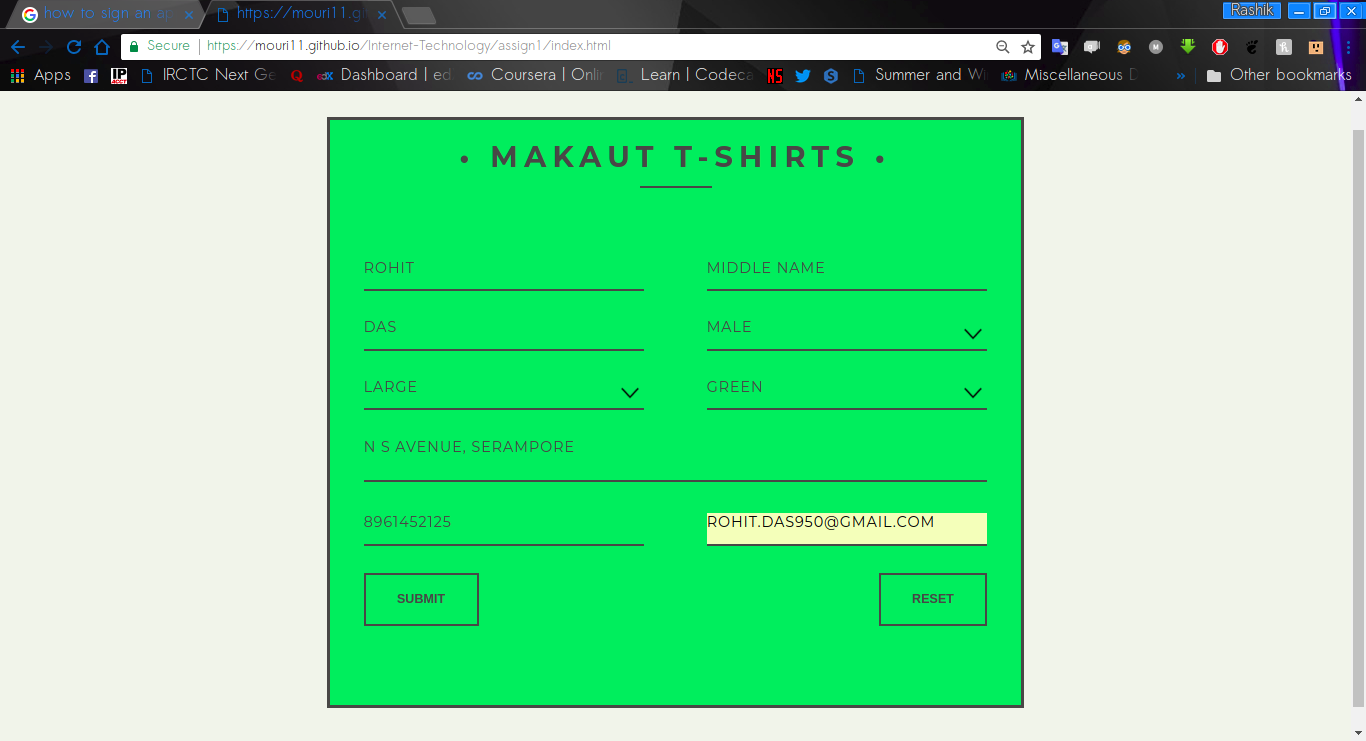
\includegraphics[width=300pt,height=\textheight,keepaspectratio]{../assign1/form1.png}
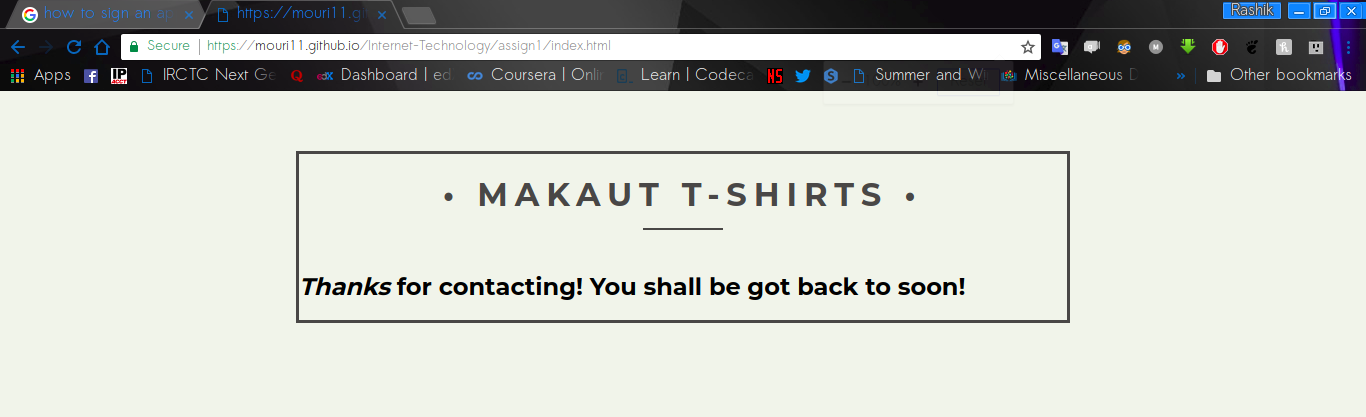
\includegraphics[width=300pt,height=\textheight,keepaspectratio]{../assign1/form2.png}
\end{figure}

\bigskip

\section{Assignment-2: Java Applets(Date: 21/4/2017)}
\subsection{Create a banner using Applet.}
\underline{Program:}
\lstinputlisting[showstringspaces=false]{../assign2/Banner/Banner.java}
\lstinputlisting[showstringspaces=false]{../assign2/Banner/Banner.html}
Output:
\begin{figure}[H]
\centering
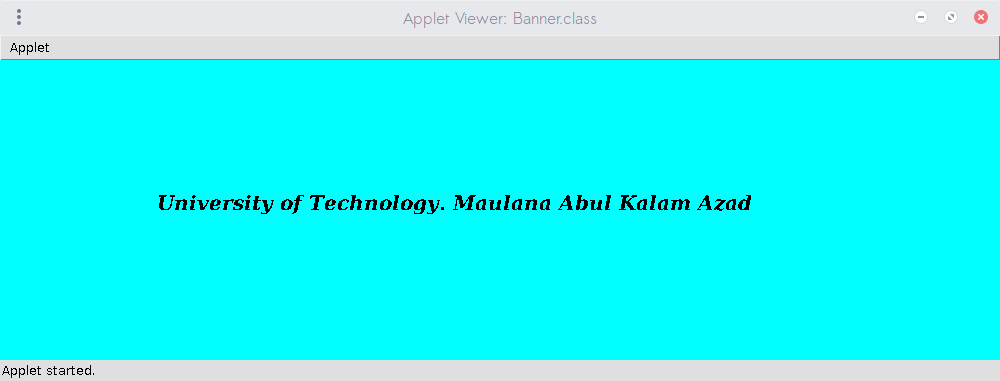
\includegraphics[width=350pt,height=\textheight,keepaspectratio]{../assign2/pics/1.png}
\end{figure}

\bigskip

\subsection{Display clock using Applet.}
\underline{Program:}
\lstinputlisting[showstringspaces=false]{../assign2/Clock/AnaClock.java}
\lstinputlisting[showstringspaces=false]{../assign2/Clock/AnaClock.html}
Output:
\begin{figure}[H]
\centering
\includegraphics[width=250pt,height=\textheight,keepaspectratio]{../assign2/pics/2.png}
\end{figure}

\bigskip

\subsection{Create different shapes using Applet.}
\underline{Program:}
\lstinputlisting[showstringspaces=false]{../assign2/Shapes/Shapes.java}
\lstinputlisting[showstringspaces=false]{../assign2/Shapes/Shapes.html}
Output:
\begin{figure}[H]
\centering
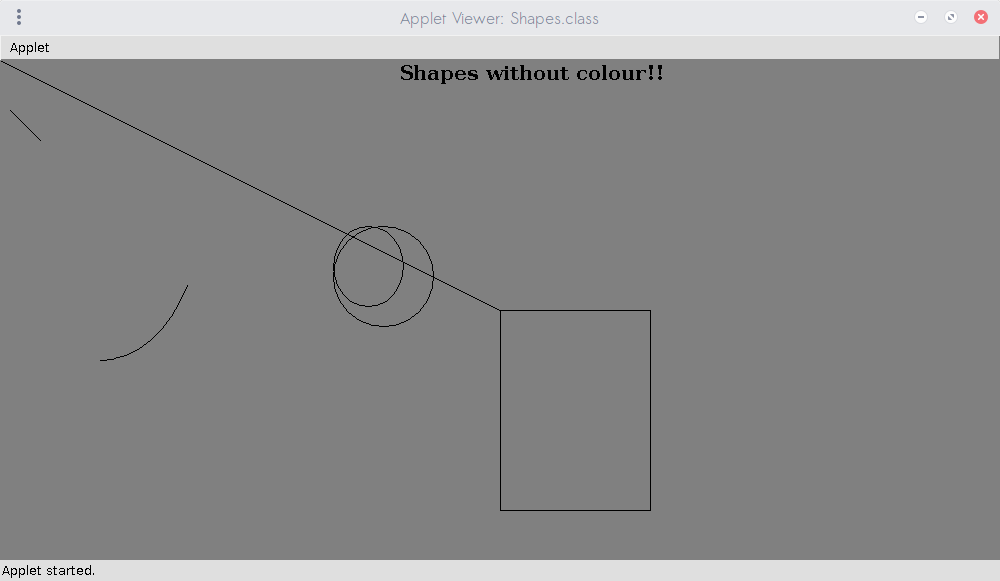
\includegraphics[width=350pt,height=\textheight,keepaspectratio]{../assign2/pics/3.png}
\end{figure}

\bigskip

\subsection{Fill colors in shapes using Applet.}
\underline{Program:}
\lstinputlisting[showstringspaces=false]{../assign2/Shapes/ColShapes.java}
\lstinputlisting[showstringspaces=false]{../assign2/Shapes/ColShapes.html}
Output:
\begin{figure}[H]
\centering
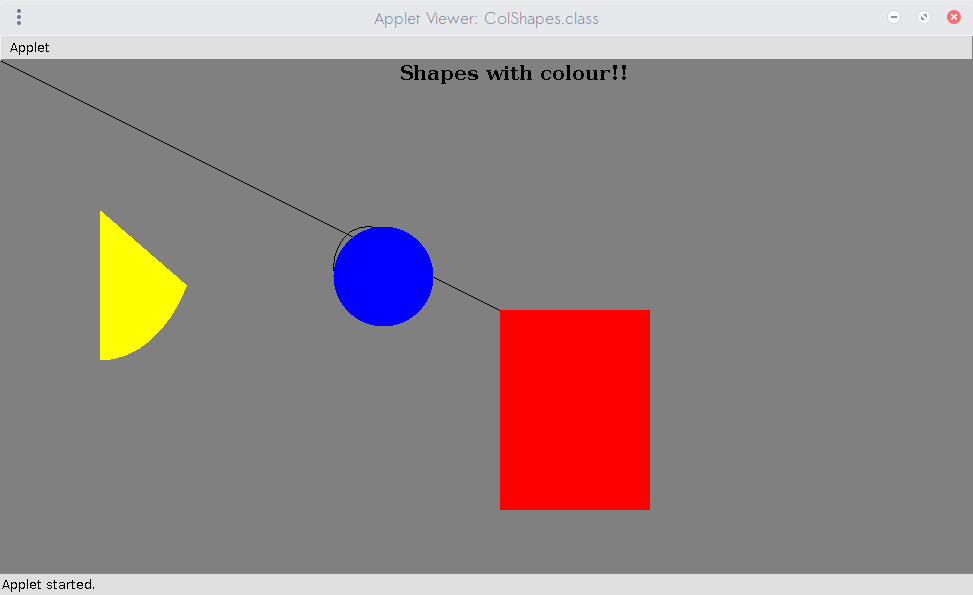
\includegraphics[width=350pt,height=\textheight,keepaspectratio]{../assign2/pics/4.png}
\end{figure}

\bigskip

\subsection{Goto a link using Applet.}
\underline{Program:}
\lstinputlisting[showstringspaces=false]{../assign2/Linker/Linker.java}
\lstinputlisting[showstringspaces=false]{../assign2/Linker/Linker.html}
Output:
\begin{figure}[H]
\centering
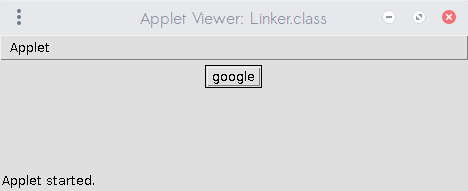
\includegraphics[width=300pt,height=\textheight,keepaspectratio]{../assign2/pics/5.png}
\end{figure}
\bigskip
\begin{figure}[H]
\centering
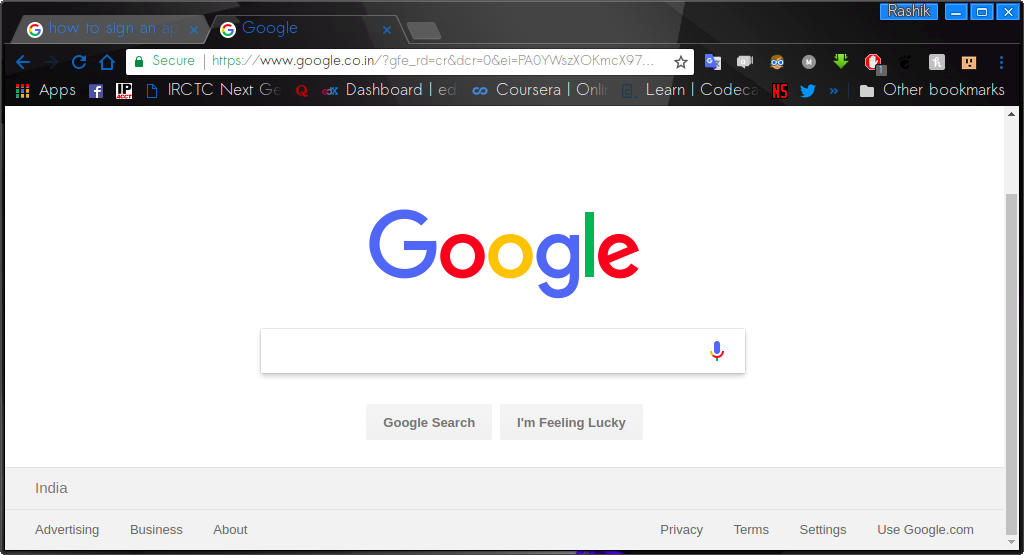
\includegraphics[width=300pt,height=\textheight,keepaspectratio]{../assign2/pics/5-1.png}
\end{figure}

\bigskip

\subsection{Create an event listener in Applet.}
\underline{Program:}
\lstinputlisting[showstringspaces=false]{../assign2/Listener/Listen.java}
\lstinputlisting[showstringspaces=false]{../assign2/Listener/Listen.html}
Output:
\begin{figure}[H]
\centering
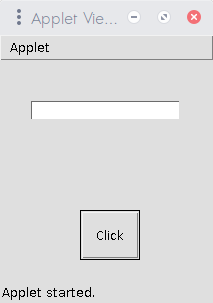
\includegraphics[width=150pt,height=\textheight,keepaspectratio]{../assign2/pics/6.png}
\end{figure}

\bigskip

\subsection{Display image using Applet.}
\underline{Program:}
\lstinputlisting[showstringspaces=false]{../assign2/Image/Imager.java}
\lstinputlisting[showstringspaces=false]{../assign2/Image/Image.html}
Output:
\begin{figure}[H]
\centering

\includegraphics[width=150pt,height=\textheight,keepaspectratio]{../assign2/pics/7.png}
\end{figure}

\bigskip

\subsection{Play sound using Applet.}
\underline{Program:}
\lstinputlisting[showstringspaces=false]{../assign2/Sound/Sound.java}
\lstinputlisting[showstringspaces=false]{../assign2/Sound/Sound.html}
Output:
\begin{figure}[H]
\centering
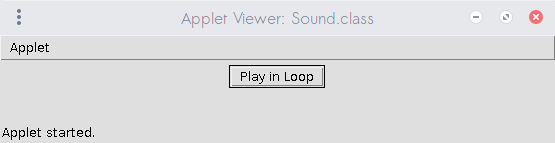
\includegraphics[width=350pt,height=\textheight,keepaspectratio]{../assign2/pics/9.png}
\end{figure}

\bigskip

\subsection{Read a file using Applet.}
\underline{Program:}
\lstinputlisting[showstringspaces=false]{../assign2/Files/Filer.java}
\lstinputlisting[showstringspaces=false]{../assign2/Files/Filer.html}
\lstinputlisting[showstringspaces=false]{../assign2/Files/test1.txt}
Output:
\begin{figure}[H]
\centering
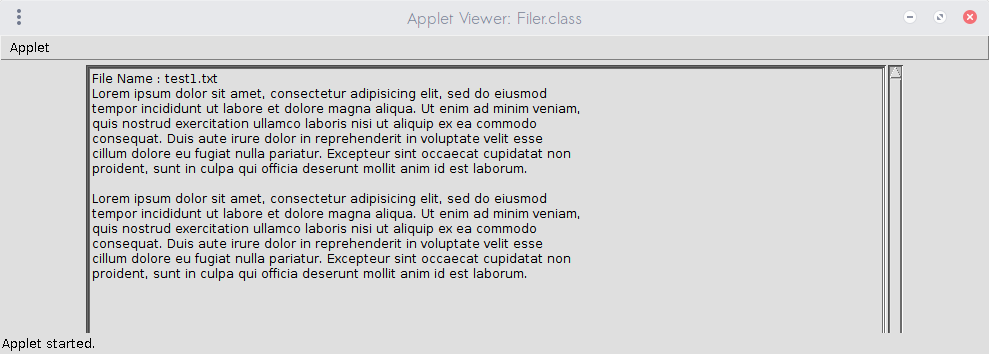
\includegraphics[width=350pt,height=\textheight,keepaspectratio]{../assign2/pics/10.png}
\end{figure}

\bigskip

\subsection{Write to a file using Applet.}
\underline{Program:}
\lstinputlisting[showstringspaces=false]{../assign2/Files/Filew.java}
\lstinputlisting[showstringspaces=false]{../assign2/Files/Filew.html}
Output:
\begin{figure}[H]
\centering
%\includegraphics[width=350pt,height=\textheight,keepaspectratio]{./pics/C/2.png}
\end{figure}

\bigskip

\end{document}